% 这里是第二章,主要介绍功能分解和总体设计思路
% 作者:谭正
% 上次更新:1.10.20.37

\chapter{功能分解和总体设计思路}

\section{功能分解}

本项目所设计的装置的目标功能可以分解为接收和分析指令、夹取不同的工件和将其移动到指定位置。

\subsection{接收和分析指令}

本装置接受到的指令需要包含夹取的工件位置列表,所需夹取的工件的类别列表等信息。
位置坐标使用笛卡尔坐标系,以本装置的基坐标为基底描述;
工件的类别用不同的字符串描述。
在本装置完成夹取装盘后,是否通知顾客取单还取决于以实时取餐区域剩余工件数量等,
所以本装置接收到得指令中应能够指示其完成夹取后的行为。

综上所述,输入本装置的指令应可用如图\ref{fig:codeblock}所示的数据结构储存。

\begin{figure}[!h]
\begin{codeblock}[language=python]
    msg = [
        ['all', [0, 0, 0]],  
        # 'all' 表示仅由该装置就可以夹取本次订单上的所有所需工件
        # 第一个元素的坐标不具有实际意义,[0, 0, 0]也是根本不可能达到的坐标
        ['cola', [1, 2, 2]],
        ['hamburger', [1, 3, 3]]
        ]
\end{codeblock}
\bicaption[输入本装置的指令结构]{输入本装置的指令结构}{Input command structure}
\label{fig:codeblock}
\end{figure}

为保证系统的稳定运行,我们拟不对用户开放设置装置运动快慢的接口。

\subsection{夹取不同的工件}

为了使我们的末端执行机构能够夹取不同形态的工件,我们在设计末端执行机构时使用了两自由度的夹取器。
举个例子,在如图\ref{fig:endeffector}所示的末端执行机构中,原动件有就有两个:跟电机输出轴相连接的轴(图\ref{fig:endeffector}中的$E, E'$)和工件的形态尺寸的对夹取作用的杆(图\ref{fig:endeffector}中的$3, 3'$)。

\begin{figure}[!htp]
    \centering
    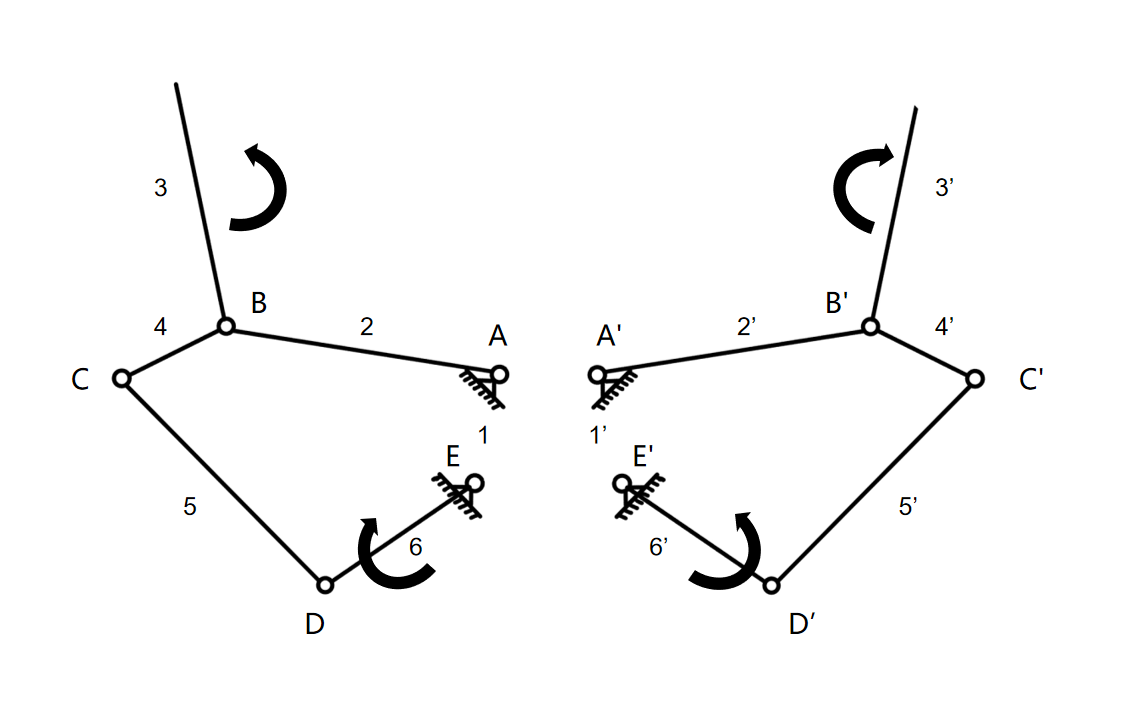
\includegraphics[width = 0.8\textwidth]{end_effector.png}
    \bicaption[五杆机构夹取器]{用五杆机构实现的末端执行机构}{End effector with five-bar mechanism}
    \label{fig:endeffector}
\end{figure}
\subsection{移动工件}

在移动工件有很多解决方案,为了方便直接改装现有的肯德基餐厅并且保留更多的可开发性,本项目在设计时放弃了诸如传送带等运输方式,而是采用一个具有多自由度的机械臂来移动工件。
考虑到在移动特殊工件(如饮料)时,机械臂的末端需要保持水平以防止液体溢出,所以我们所设计的机械臂应有一个冗余的自由度,而移动工件的空间坐标$(x, y, z)$至少需要3个自由度,所以我们所设计的机械臂至少需要4个自由度。

\hfill

根据上述功能分解,为了满足我们对肯德基快餐的分装传送需求,我们给出的解决方案为:一个四自由度的机械臂加一个自适应末端执行机构。

\section{运动转换的基本功能和传动、减速机构的选型}

\subsection{运动类型的转化}

在本装置中,四自由度机械手的是一个位置随动的开环控制系统,各个关节的转动由步进电机就可以驱动,通过发送脉冲可控制其转动到指定角度。因此在这一部分,原动件运动类型为转动(周转、摆动),从动件的运动类型为摆动,所以运动类型不需要要转化;而在本装置的末端执行机构中,需要将原动件的转动转化为夹取运动,采用图\ref{fig:endeffector}所示的五杆机构就可以实现这种转化。

\subsection{机构选型}

设计时需要我们进行选型的机构主要是传动、减速机构,选择的依据如下:
\begin{enumerate}
    \item   根据从动件的运动轨迹(不与实际设计的机架相干涉)选择末端执行机构;
    \item   根据市面上方便买到的电机的功率、额定扭矩和我们所大致需要的扭矩选择我们的减速机构。
\end{enumerate}


\section{工作流程}

根据上述分析可以绘制本装置的工作流程图如图\ref{fig:work_flow}。
其中,机械臂运动的可以用工作流程图可以表示如图\ref{fig:robot_move}。
在提取下一时刻各个关节位置时,若已经到达运动轨迹终点,则下一时刻各关节位置与当前相同。

\begin{figure}[!htp]
    \centering
    \resizebox{\textwidth}{!}{\begin{tikzpicture}[node distance=5cm]
    \node (track) [startstop] {收到运动轨迹信息};
    \node (get_angles) [io, right of=track, align=center] {提取下一时刻 \\ 各个关节位置};
    \node (move) [process, right of=get_angles, align=center] {控制各个关节 \\ 向目标位置运动};
    \node (finish) [decision, right of=move, align=center] {是否到达 \\ 轨迹终点};
    \node (notify) [startstop, right of=finish, align=center] {通知上位机已到 \\ 达轨迹终点};
    \node (anc_one) [above of=finish, yshift=-3cm] {};
    \node (anc_two) [above of=get_angles, yshift=-3cm] {};
    %连接具体形状
    \draw [arrow] (track) -- (get_angles);
    \draw [arrow] (get_angles) -- (move);
    \draw [arrow] (move) -- (finish);
    \draw [arrow] (finish) -- node [anchor=north] {是} (notify);
    \draw [arrow] (finish) -- (anc_one);
    \draw [arrow] (anc_one) -- node [anchor=south] {不论是否} (anc_two);
    \draw [arrow] (anc_two) -- (get_angles); 
\end{tikzpicture}
}
    \bicaption[机械臂运动流程图]{机械臂运动流程图}{Robotic arm moving flow chart}
    \label{fig:robot_move}
\end{figure}

\begin{figure}[!htp]
    \centering
    \resizebox{6cm}{!}{\begin{tikzpicture}[node distance=2cm]
    \node (order) [startstop] {顾客下单};
    \node (get_msg) [io, below of=order] {提取工件种类、位置信息};
    \node (move1) [process, below of=get_msg, align=center] {控制末端执行机构运动到 \\ 工件摆放位置};
    \node (get) [process, below of=move1] {夹取工件};
    \node (move2) [process, below of= get, align=center] {控制末端执行机构运动到 \\ 工件目的地};
    \node (place) [process, below of= move2] {放置工件};
    \node (finish) [decision, below of=place, align=center, yshift=-1cm] {判断是否 \\ 移动完毕};
    \node (left) [decision, right of=finish, align=center, xshift=3cm] {判断是否还有 \\ 剩余工件要移动};
    \node (notify) [startstop, below of=finish, yshift=-1.5cm] {通知顾客取单};
    \node (not_notify) [startstop, right of=notify, align=center, xshift=3cm] {等待工作人员 \\ 通知顾客取单};
    \node (reset) [startstop, below of=notify] {机械臂返回初始位置};
    %连接具体形状
    \draw [arrow](order) -- (get_msg);
    \draw [arrow](get_msg) -- (move1);
    \draw [arrow](move1) -- (get);
    \draw [arrow](get) -- (move2);
    \draw [arrow](move2) -- (place);
    \draw [arrow](place) -- (finish);
    \draw [arrow](finish) -- node[anchor=east] {是} (notify);
    \draw [arrow](finish) -- node[anchor=north] {否} (left);
    \draw [arrow](left) |- node[anchor=west] {是} (get_msg);
    \draw [arrow](left) -- node[anchor=west] {否} (not_notify);
    \draw [arrow](notify) -- (reset);
    \draw [arrow](not_notify) |- (reset);
\end{tikzpicture}
}
    \bicaption[本装置的总工作流程图]{总工作流程图}{Overall workflow}
    \label{fig:work_flow}
\end{figure}

